\chapter{Expected Results}

\label{ch: Res}

The expected result of this work is a software capable of correctly estimating the parameters of Type-3 WTG's mathematical model. To do so, the software will apply the proposed estimation method comprises of MVMO and TSM methods combined. 

The measurements will be obtained from a small power system simulated on specific software, such as DIgSILENT or MATLAB. At first, the model proposed in \cite{Erlich2012} will be employed, but it can be further changed if needed. Also, other estimation methods, such as Particle Swarm Optimization, Differential Evolution or Kalman Filters, may be implemented for comparison purposes.

\section{Partial Results}

The hybrid approach for parameters estimation presented in this work is already implemented and have shown great results for models. As depicted in Figure \ref{fig: spring-mass}, the proposed method can correctly identify the parameters of a spring-mass system. The same application was employed on load model identification and is subject of a paper presented by the author on the 2019 Canadian Conference on Electrical and Computer Engineering.

\begin{figure}[h]
	\caption{Results of method for spring-mass system}
	\begin{center}
		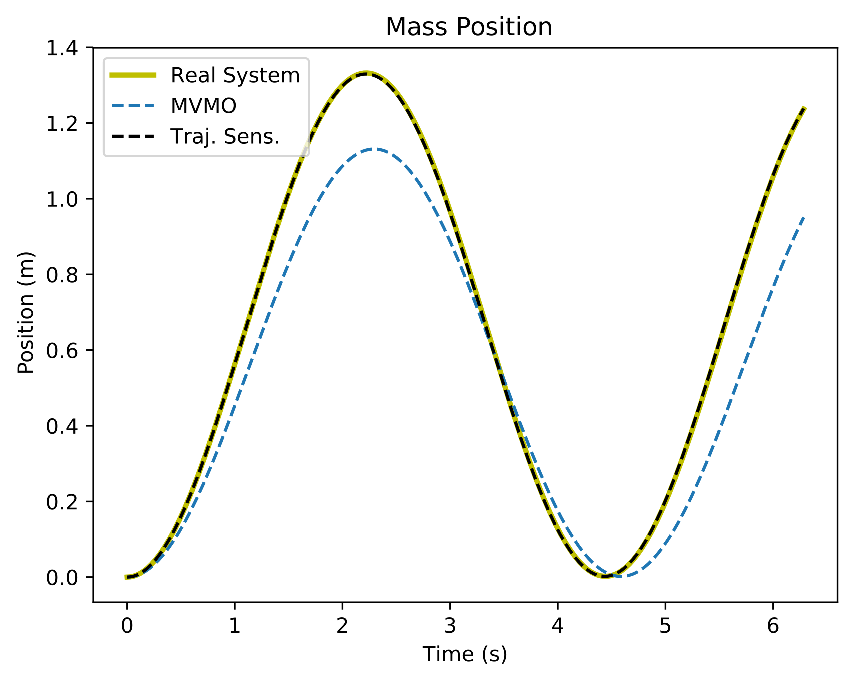
\includegraphics[scale=0.5]{Images/SpringMass.eps}
	\end{center}
	\label{fig: spring-mass}
\end{figure}

\section{Work Progress}

With the methods already implemented and tested, the focus now is on the DFIG model. The model has presented some results, but it is not accurate as required, requesting some studies about this topic. Also, the GUI is under development and already has some features implemented using Python's library Tkinter. A proposal to also develop features using Qt, a different GUI tool package, is currently under consideration.